\PassOptionsToPackage{svgnames}{xcolor}
\documentclass[10pt,letterpaper]{article}
\usepackage[top=.25in, bottom=.5in, left=.5in, right=.5in]{geometry}
\usepackage{tcolorbox}
\usepackage{lipsum}
\tcbuselibrary{skins,breakable}
\usetikzlibrary{shadings,shadows}

\usepackage{graphicx} % Allows to include images
\usepackage{booktabs} % Allows the use of \toprule, \midrule and \bottomrule in tables

\usepackage{multicol}
\usepackage{float}

\usepackage[T1]{fontenc}
\usepackage[utf8]{inputenc}

\usepackage{hyperref}

\title{Practice 3: Iron Curtain Defense}
\author{}
\date{}

\newenvironment{agendablock}[1]{%
    \tcolorbox[beamer,%
    noparskip,breakable,
    colback=LightGray,colframe=DarkGray,%
    colbacklower=Gray!75!LightGray,%
    title=#1]}%
    {\endtcolorbox}

\newenvironment{evenBlock}[1]{%
    \tcolorbox[beamer,%
    noparskip,breakable,
    colback=LightGreen,colframe=DarkGreen,%
    colbacklower=LimeGreen!75!LightGreen,%
    title=#1]}%
    {\endtcolorbox}

\newenvironment{oddBlock}[1]{%
    \tcolorbox[beamer,%
    noparskip,breakable,
    colback=LightBlue,colframe=DarkBlue,%
    colbacklower=DarkBlue!75!LightBlue,%
    title=#1]}%
    {\endtcolorbox}

\newenvironment{myexampleblock}[1]{%
    \tcolorbox[beamer,%
    noparskip,breakable,
    colback=LightGreen,colframe=DarkGreen,%
    colbacklower=LimeGreen!75!LightGreen,%
    title=#1]}%
    {\endtcolorbox}

\newenvironment{myalertblock}[1]{%
    \tcolorbox[beamer,%
    noparskip,breakable,
    colback=LightCoral,colframe=DarkRed,%
    colbacklower=Tomato!75!LightCoral,%
    title=#1]}%
    {\endtcolorbox}

\newenvironment{myblock}[1]{%
    \tcolorbox[beamer,%
    noparskip,breakable,
    colback=LightBlue,colframe=DarkBlue,%
    colbacklower=DarkBlue!75!LightBlue,%
    title=#1]}%
    {\endtcolorbox}

\usepackage{lmodern}

\begin{document}
\fontfamily{lmss}\selectfont
\maketitle

\begin{agendablock}{Practice Activities}
    Dribbling and Ball Control at your feet is another key skill.  The ability to dribble well allows you to find open space to pass or shoot. 
    \begin{enumerate}
        \item Warm ups / Coerver Touches [ 15 min ]
        \item Agility Runs [ 24 min ]
        \item Defensive Drills [ 18 min ]
        \item Game Situational Drills [ 15 min ]
        \item Small Sided Game [ 15 min ]
    \end{enumerate}
\end{agendablock}

\begin{agendablock}{Captain Led Warm ups / Coerver Touches (15 min) }
    \textbf{Warmups}
    \begin{enumerate}
        \item Jog to the 18 yard line and back twice with your ball (inside cut first time, outside cut the second),
        \item Side-Step to 18 yd line and back twice,
        \item Butt Kickers to the 18 yd line and back twice,
        \item Jog Backwards to the 18 yd line and back twice.
    \end{enumerate}
    \textbf{Touches}
    \begin{enumerate}
        \item Toe-Touches (20 count alternating feet).
        \item Pull back and Push Forward (10 each foot).
        \item Side to Side or Pendulums (20 count).
        \item Triangles (10 each foot).
        \item Pullback-Behind (20 count).
    \end{enumerate}
\end{agendablock}

\clearpage



\section{Agility Runs}
\href{https://www.youtube.com/watch?v=3ew2m3m5f0M}{Agility Runs} () (10 min)
Defenders and forwards needs to be agile, stop and go hard, these exercises will work on speed and agility.

\textbf{Time: 6 minutes}
%\begin{evenBlock}{Gate Dribbling (10 min)}
%Set up 3 gates in a zig-zag pattern about 6 to 10 yards apart.  The gates should be about a yard wide or less depending on dribbling skill of the group.  Players start a the end line and dribble through the gates as fast as possible.  Use the same technique as the previous drill.
%\end{evenBlock}

\begin{oddBlock}{De-Acceleration Shuddle}

\begin{minipage}[t]{\linewidth}
    \centering
    
    \begin{minipage}{.3\linewidth} % Left column and width
        %\begin{figure}
            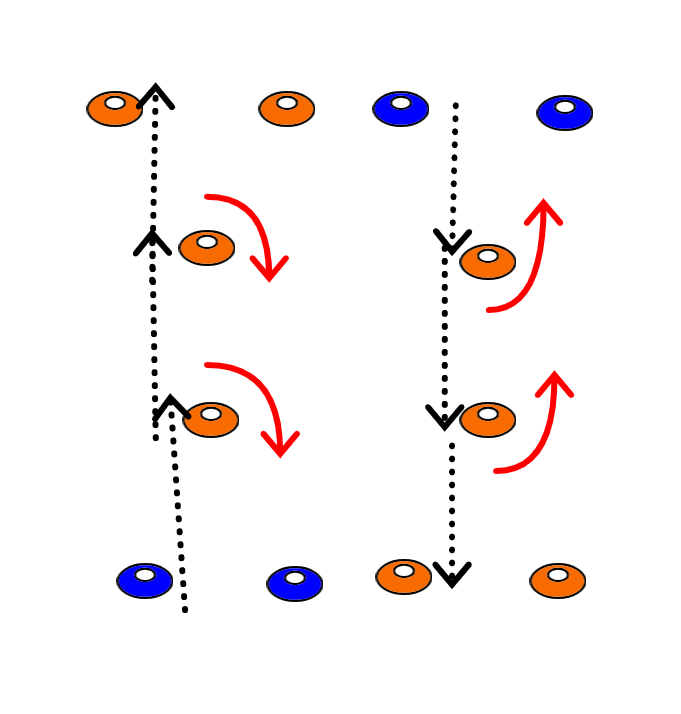
\includegraphics[width=\textwidth]{../img/Trimmed/deaccel_shuddle}
        %    \caption{Drill: 4 Person Passing}
        %\end{figure}
    \end{minipage}
    \hspace{0.05\linewidth}
    \begin{minipage}{.6\linewidth} % Left column and width
        \textbf{Drill Description:}
        This is an agility drill to practice both acceleration and de-acceleration.
        \begin{enumerate}
        \setlength{\itemsep}{0pt}
        \setlength{\parskip}{0pt}
        \setlength{\parsep}{0pt}
        \item Players start at blue gate
        \item Then run to the left hand side of the first orange cone and while facing forward shuddle around the cone using at least 6 quick toe taps.
        \item Then accelerate to the left of the next orange cone and shuddle around the cone then finish with a full acceleration through the orange gate.
        \item A second line forms behind the other blue cone and the drill repeats but this time one races to the right hand side of the cones and shuddle around to the left.
        \item Repeat each set 4 times.
        \end{enumerate}
    \end{minipage}
\end{minipage}
    \vspace{12pt}
    
    \textbf{Coaching Points:}
    \begin{itemize}
        \setlength{\itemsep}{0pt}
        \setlength{\parskip}{0pt}
        \setlength{\parsep}{0pt}
        \item Focus on quickly getting to speed then slowing down.
        \item Focus on using small quicks touches around the cone, keeping it tight.
        \item Stay low and use your bend legs to explode away,
        \item Then compress them to slow down.
        \item Finish strong by sprinting right through the last gate, jogging back to the next blue gate.
    \end{itemize}
\end{oddBlock}

\textbf{Time: 6 minutes}
%\begin{evenBlock}{Gate Dribbling (10 min)}
%Set up 3 gates in a zig-zag pattern about 6 to 10 yards apart.  The gates should be about a yard wide or less depending on dribbling skill of the group.  Players start a the end line and dribble through the gates as fast as possible.  Use the same technique as the previous drill.
%\end{evenBlock}

\begin{oddBlock}{Cross-Hairs}

\begin{minipage}[t]{\linewidth}
    \centering
    
    \begin{minipage}{.2\linewidth} % Left column and width
        
        \centering
        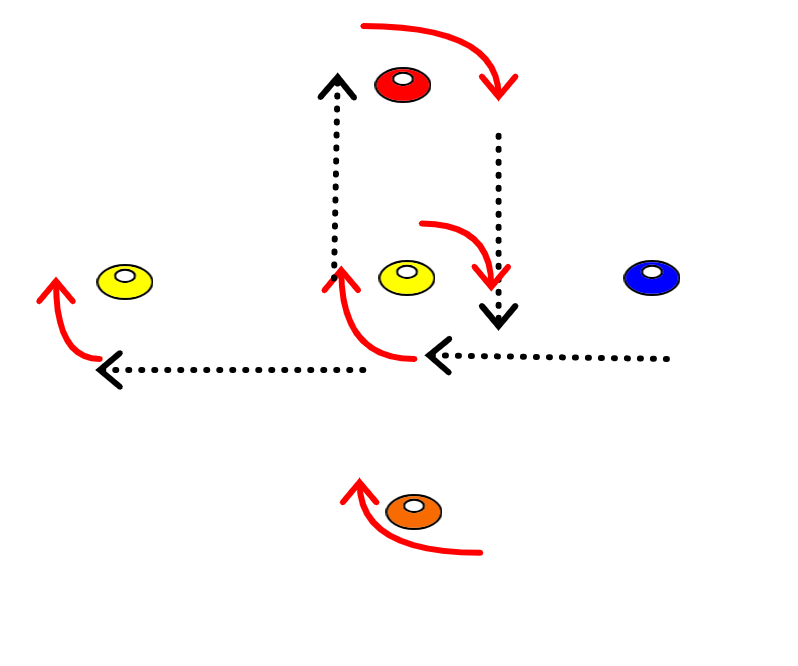
\includegraphics[width=\textwidth]{../img/Trimmed/cross_hairs}

    \end{minipage}
    \hspace{0.05\linewidth}
    \begin{minipage}{.7\linewidth} % Left column and width
        \textbf{Drill Description:}
        
        \begin{enumerate}
        \setlength{\itemsep}{0pt}
        \setlength{\parskip}{0pt}
        \setlength{\parsep}{0pt}
        \item Players start at blue cone and race to the center cone turn right and race around the outer cones and always returning to the center cone.
        \item Finish by accelerating past the blue cone.
        \end{enumerate}
    \end{minipage}
\end{minipage}
%\vspace{12pt}
%
%    \textbf{Coaching Points:}
%    \begin{itemize}
%        \setlength{\itemsep}{0pt}
%        \setlength{\parskip}{0pt}
%        \setlength{\parsep}{0pt}
%        \item
%    \end{itemize}

\end{oddBlock}

\textbf{Time: 6 minutes}
%\begin{evenBlock}{Gate Dribbling (10 min)}
%Set up 3 gates in a zig-zag pattern about 6 to 10 yards apart.  The gates should be about a yard wide or less depending on dribbling skill of the group.  Players start a the end line and dribble through the gates as fast as possible.  Use the same technique as the previous drill.
%\end{evenBlock}

\begin{oddBlock}{Lateral Shuttle}

\begin{minipage}[t]{\linewidth}
    
    \begin{minipage}{.2\linewidth} % Left column and width
        \centering
        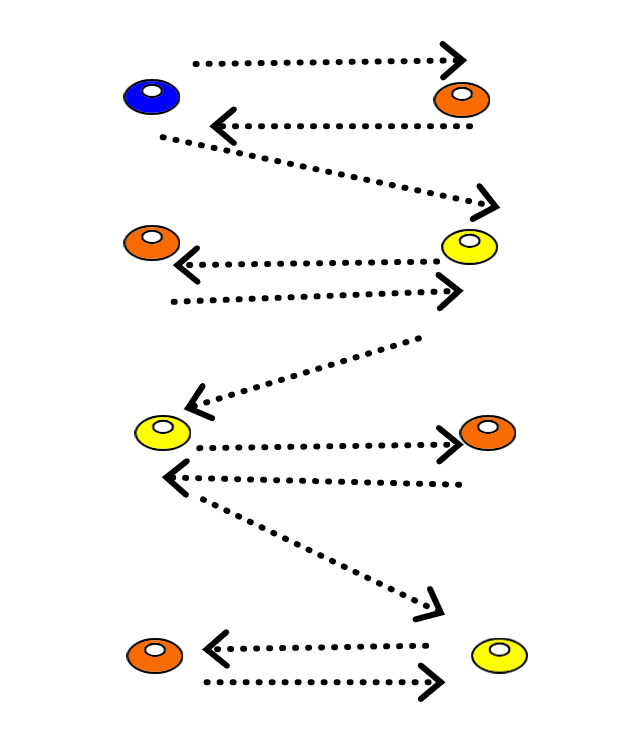
\includegraphics[width=\textwidth]{../img/Trimmed/lateral_shuddle}
    \end{minipage}
    \hspace{0.05\linewidth}
    \begin{minipage}{.7\linewidth} % Left column and width
        \textbf{Drill Description:}
        This agility drill works on lateral shuffling a critical skill for defenders. 
        \begin{enumerate}
            \setlength{\itemsep}{0pt}
            \setlength{\parskip}{0pt}
            \setlength{\parsep}{0pt}
            \item Players start at blue gate facing the line of 3 cones ahead of him,
            \item They shuttle side-ways to the orange cone, touch it with a finger then shuttle back to the blue cone touching it.
            \item Shuttle to diagonally to the yellow cone then to the orange cone, touching it, and back then to the yellow cone touching it, then shuttle diagonally to the next yellow cone.
            \item Keep repeating until the end.
        \end{enumerate}
    \end{minipage}
\end{minipage}
    %\vspace{12pt}
    %
    %\textbf{Coaching Points:}
    %\begin{itemize}
    %    \setlength{\itemsep}{0pt}
    %    \setlength{\parskip}{0pt}
    %    \setlength{\parsep}{0pt}
    %    \item TBD
    %\end{itemize}
\end{oddBlock}

\clearpage

\section{Drills}

\textbf{Time: 6 minutes}  Requires 5-10 cones per pair of players.
\begin{evenBlock}{Frogger}

\begin{minipage}[t]{\linewidth}
    \centering
    
    \begin{minipage}{.3\linewidth} % Left column and width
        %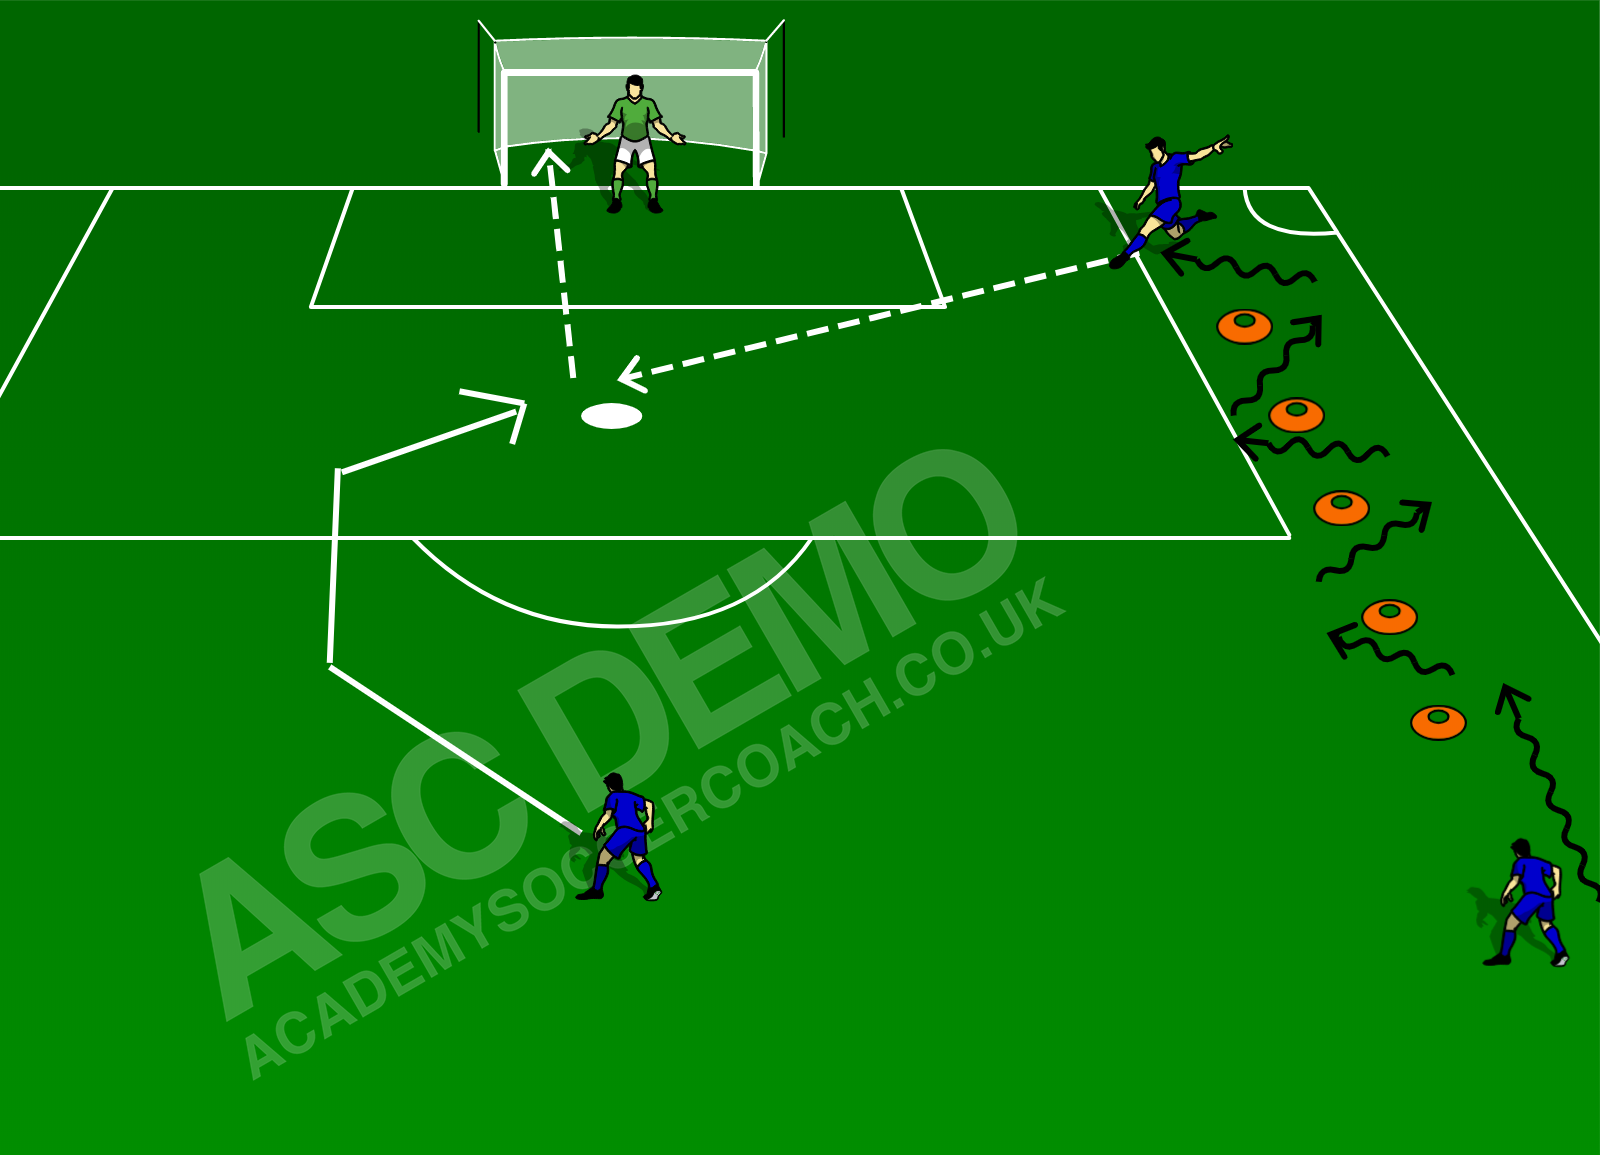
\includegraphics[width=\textwidth]{../img/Trimmed/Dribble-Cross-Shoot}
    \end{minipage}
    \hspace{0.05\linewidth}
    \begin{minipage}{.6\linewidth} % Left column and width
        \textbf{Drill Description:}
        \begin{enumerate}
        \setlength{\itemsep}{0pt}
        \setlength{\parskip}{0pt}
        \setlength{\parsep}{0pt}
        \item 4 1x1 yard boxes are setup.
        \item 1 Player is on the outside of the long edge.
        \item 1 player is inside the boxes.
        \item The outside player is trying to cross through a box before the inside player can get his foot planted inside box.
        \item Players switch roles often and rotate the players.
        \end{enumerate}

        \vspace{10pt}
        
        \textbf{Coaching Points:}
        \begin{itemize}
        \setlength{\itemsep}{0pt}
        \setlength{\parskip}{0pt}
        \setlength{\parsep}{0pt}
        \item Player inside the box is the defender and using a lateral move to block the other player.
        \item Both players should be on their toes all the time to increase reaction time.
        \end{itemize}

    \end{minipage}
\end{minipage}

\end{evenBlock}

\textbf{Time: 5 minutes} Requires 4 cones per pair of players.
\begin{evenBlock}{Back-Petal}
Instruct how to move backward and apply pressure.

\textbf{Goal for the Drill:}

For the Defender to learn how to effectively back-petal to keep pressure on the attacker but not allow him to pass the defender.


\textbf{How:}

Create a 10 yard box.  The attacker starts at one box edge and dribbles out the other box edge, but trys to get past the defender.  The attacker can't dribble out the sides of the box.

The defender back petals trying to keep the attacker in front of him and not letting him get past him.  The defender should try to force the attacker to the edges of the box.

The defender does not try to steal or block the ball - focus on the attacker.

Switch roles, then rotate around.  So players can be attackers and defenders against the other players.

\textbf{Coaching Points:}
\begin{itemize}
    \item Staggered stance with toes at a 45 degree angle.
    \item Bent knees with weight on the balls of the feet.
    \item Chest leaning over the toes.
    \item Low center of gravity for greater explosion/quick change of direction (upright takes longer to start).
    \item Ability to shuffle quickly.
    \item Shuffle backward  angling your body to force them one direction or the other.  This simulates pushing them away from center of the field (away from our the goal).
\end{itemize}

\end{evenBlock}

\textbf{Time: 10 minutes} Uses same setup as previous drill.
\begin{evenBlock}{Box Defending}
Create a 10 yard box.  The defender (D1) starts within the box, and a second player the attacker (A1) attempts to dribble past the defender to the other side of the box.

If A1 dribbles the ball out the far end - he wins and the defender stays in the box and trys to defend the next attacker.

If D1 is able to take control or kick the ball out of the sides of the box - he wins.
Then A1 becomes the defender and D1 goes to the back of Attacking Line.

Once a player wins the next attacker trys to get through.  This makes the defender transition quickly.

\textbf{When defending 1v1’s in soccer it is very important to focus on the following key elements}:
\begin{itemize}
\item Staggered stance with toes at a 45 degree angle.
\item Bent knees with weight on the balls of the feet.
\item Chest leaning over the toes.
\item Low center of gravity for greater explosion/quick change of direction (upright takes longer to start).
\item Ability to shuffle quickly.
\item Pay attention to the distance of pressure (depends on speed of attacker vs. the speed of the defender) usually 1-3 yards
\item Remember that the player closest to the attacker should be the player pressuring the ball. Players should sprint to close down space as quickly as they can, then when they get 5 yards from the attacker they should slow down and take steps backwards to match the pace of the attacker. During this time, the defender should slowly close down the space between the attacker and defender. Often proper pressure will cause the attacker to lose the ball.

One way to have players recall the proper way to defend is by the term “Quick, Slow, Sideways, Low”.
\end{itemize}
\end{evenBlock}


%\begin{evenBlock}{Foot Soldiers (10 min)}

\begin{minipage}[t]{\linewidth}
    \centering
    
    \begin{minipage}{.4\linewidth} % Left column and width
        \centering
        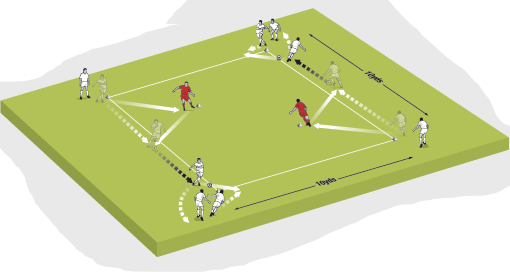
\includegraphics[width=\textwidth]{../img/Trimmed/FootSoldiers1}
        \vspace{6pt}
        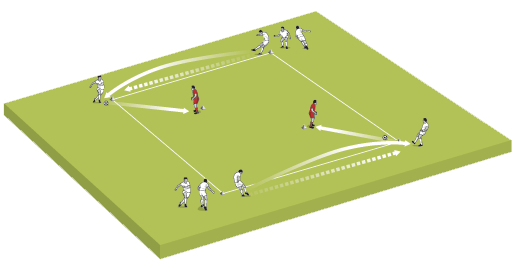
\includegraphics[width=\textwidth]{../img/Trimmed/Footsoldiers2}
    \end{minipage}
    \hspace{0.05\linewidth}
    \begin{minipage}{.5\linewidth} % Left column and width
        \textbf{Drill Description:}
        To use this simple warm-up mark out a 10x10-yard square with cones. Position a cone as shown for the central players. We have used 14 players in this activity, including two servers. You need balls and cones.
        \begin{enumerate}
        \setlength{\itemsep}{0pt}
        \setlength{\parskip}{0pt}
        \setlength{\parsep}{0pt}
        \item Place the two servers inside the square and arrange the remaining players around the four corners of the area use the central players to make one-two wall passes on opposite sides of the square and a first-time pass along the other sides of the square.
        \item Players should sidefoot their passes to the central players, who must make sure that they control the ball and pass it back to the running players so they don’t have to break their stride.
        \item You should swap the players over regularly, changing the two central wall passers. You must have two balls in play at once.
        \end{enumerate}

        \begin{enumerate}
        \setlength{\itemsep}{0pt}
        \setlength{\parskip}{0pt}
        \setlength{\parsep}{0pt}
        \item Play starts on both sides with a pass to the server who plays a one-two with the working player
        \item The player dribbles towards the cone and passes to the player at the cone
        \item The player at the next cone must be on the move to receive the ball and make a one touch pass to the next cone
        \item Players must follow the pass and keep moving around the square
        \item The receiving player for the one-two pass can take two touches because this needs to be an accurate move with a good weight on the pass
        \end{enumerate}

    \end{minipage}
\end{minipage}

\end{evenBlock}

% \clearpage
\section{Game Situational Practice}

\textbf{Time: 15 minutes}
\begin{evenBlock}{Secure the Box}

\begin{minipage}[t]{\linewidth}
    \centering
    
    \begin{minipage}{.3\linewidth} % Left column and width
        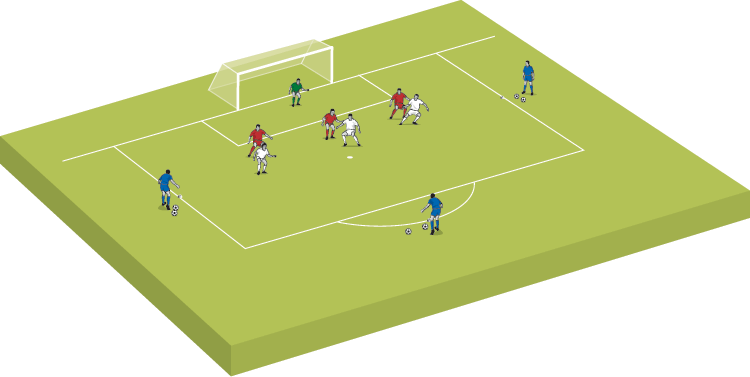
\includegraphics[width=\textwidth]{../img/Trimmed/SecureTheBox1}
    \end{minipage}
    \hspace{0.05\linewidth}
    \begin{minipage}{.6\linewidth} % Left column and width
        \textbf{Drill Description:}
        This drill is ideally played with 9 players, with 3 players per team.  With unbalanced numbers a 4th attacker could be added to create a 4v3 situation to make it harder on the defense (since this is a defensive drill).
        \begin{enumerate}
            \setlength{\itemsep}{0pt}
            \setlength{\parskip}{0pt}
            \setlength{\parsep}{0pt}
            \item The defending team must man mark, with each player picking up an attacker.
            \item The players on the edge of the area have two balls each to pass to the attackers.
            \item The serving players must pass into an attacker who is open (unmarked).
        \end{enumerate}
        
        \textbf{Coaching Points:}
        \begin{itemize}
            \setlength{\itemsep}{0pt}
            \setlength{\parskip}{0pt}
            \setlength{\parsep}{0pt}
            \item Explain marking a player is to remain within 2 or 3 feet of the attackign player.
            \item Explain how to mark a player goal side (defender between the attacker and goal).
            \item Explain how to mark a player ball side (defender between the attacker and the ball).
            \item Explain how to mark a player both goal side and ball side - defender marks the attacker goal side but is a few feet (steps) closer to the ball than the attacker.
            \item Attackers try to lose their marks.  Defenders stay marking the attacker.
            \item Defenders should communicate if they want to defend a zone or a man.  Explain to them how this can work.
            \item If zone defense is too difficult at this stage force them to play man coverage - always marking the same attacker.
        \end{itemize}

    \end{minipage}
\end{minipage}

\end{evenBlock}

%\begin{evenBlock}{2 vs. 1 Offense (10 min)}


\begin{minipage}[t]{\linewidth}
    \centering
    
    \begin{minipage}{.3\linewidth} % Left column and width
        %\begin{figure}
            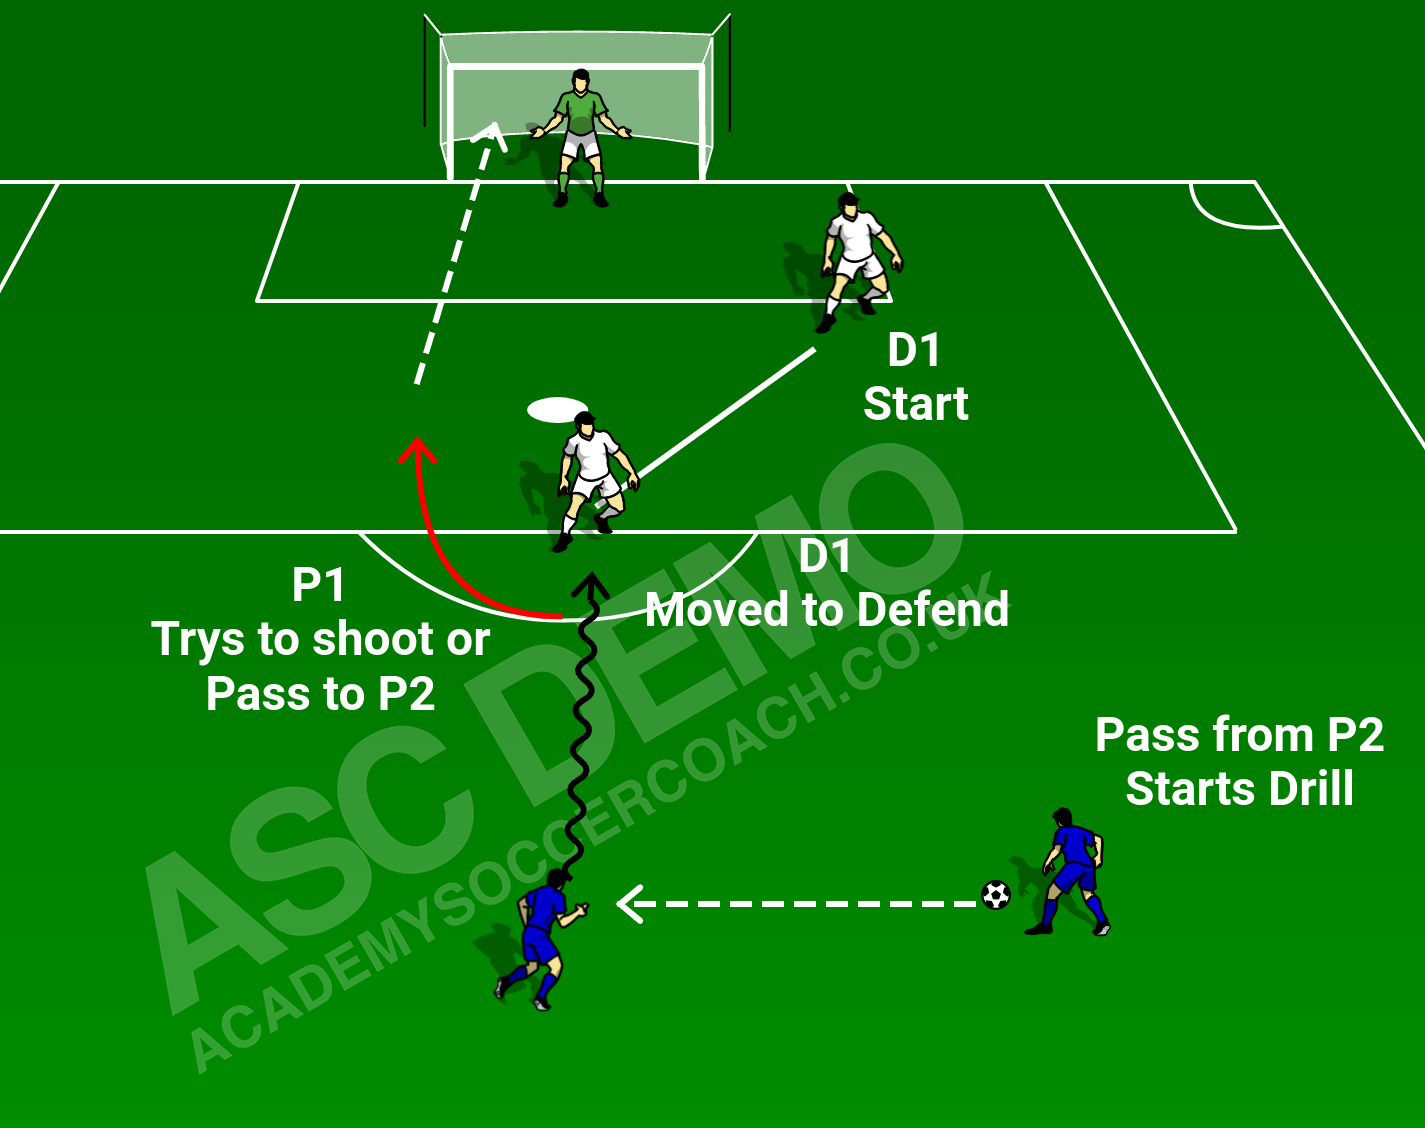
\includegraphics[width=\textwidth]{../img/Trimmed/2v1_Option}

            \vspace{3pt}
            
            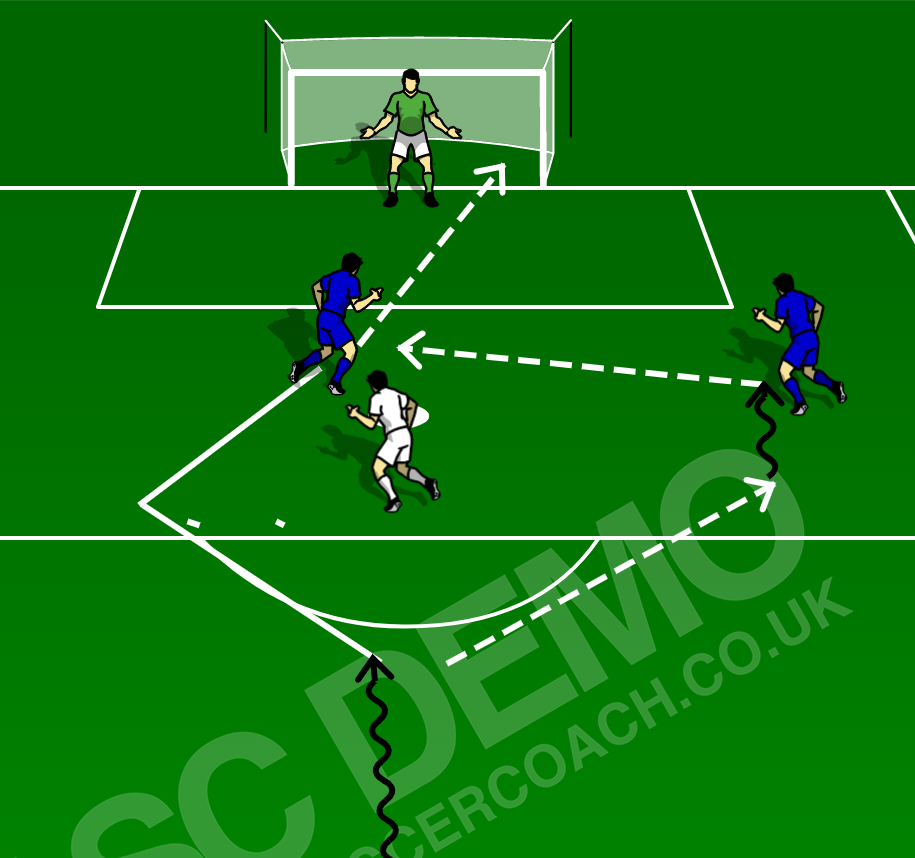
\includegraphics[width=\textwidth]{../img/Trimmed/2v1_Option_Pass}
        %    \caption{Drill: 4 Person Passing}
        %\end{figure}
    \end{minipage}
    \hspace{0.05\linewidth}
    \begin{minipage}{.6\linewidth} % Left column and width
        \textbf{Drill Description:}
        This drill is designed train the forward to make a quick decision on how to beat a defender.  He has two options, dribble around the defender or pass to his wing and make a move around the defender. 
        \begin{enumerate}
        \setlength{\itemsep}{0pt}
        \setlength{\parskip}{0pt}
        \setlength{\parsep}{0pt}
        \item The wing (P2) starts the play by passing to the forward.  The defender (D1) starts at the corner of the 6 yard box.
        \item The forward drives to goal as a defender come charging to defend.
        \item The forward has two choices, pass or make a move/touch around the defender.
        \item The goal is to get a shot on goal.
        \item If he passes the ball, the wing should cross the ball quickly as the striker is passing the defender.
        \end{enumerate}

        \vspace{3pt}
        
        Rotate rolls each shot: P2 to P1, P1 to D1, D1 to P2.

        \vspace{10pt}
        
        \textbf{Coaching Points:}
        \begin{itemize}
        \setlength{\itemsep}{0pt}
        \setlength{\parskip}{0pt}
        \setlength{\parsep}{0pt}
        \item The forward needs to decide quickly which option he plans to take.
        \item The wing needs to be ready at all times and should stay `on-side'.
        \item The forward should try and take advantage of any weakness of the defense, or try and create weakness by using a scissor move or a fake.
        \item Explain on-sides and off-sides.
        \end{itemize}

    \end{minipage}
\end{minipage}

\end{evenBlock}

\section{Game Time}

\textbf{Time: 15 minutes}
\begin{oddBlock}{Small Sided Game}
    \textbf{Recap Positioning from P1}
\end{oddBlock}

If not enough players for a game try this drill:
\begin{evenBlock}{Press \& Protect}

\begin{minipage}[t]{\linewidth}
    \centering
    
    \begin{minipage}{.4\linewidth} % Left column and width
        \centering
        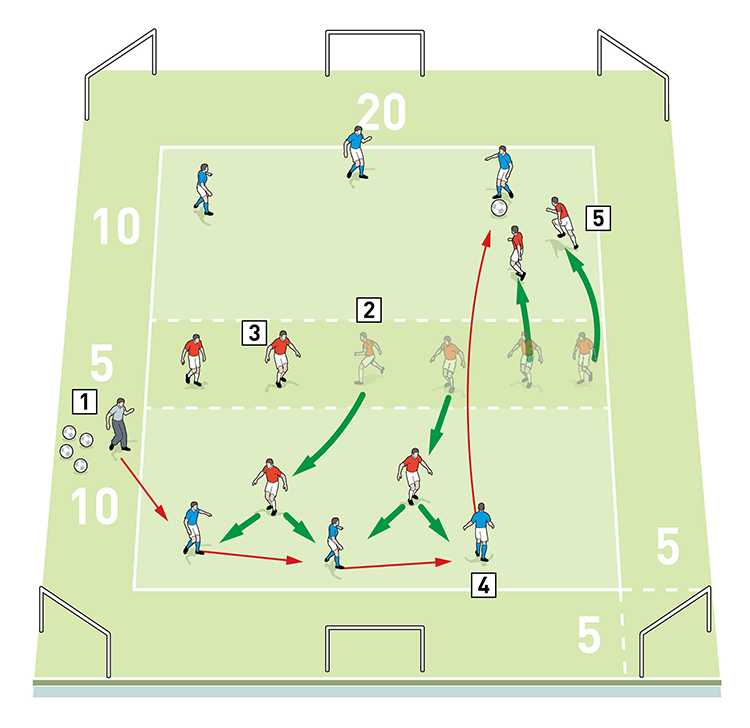
\includegraphics[width=\textwidth]{../img/Trimmed/Press_Protect}

        \vspace{6pt}
        
        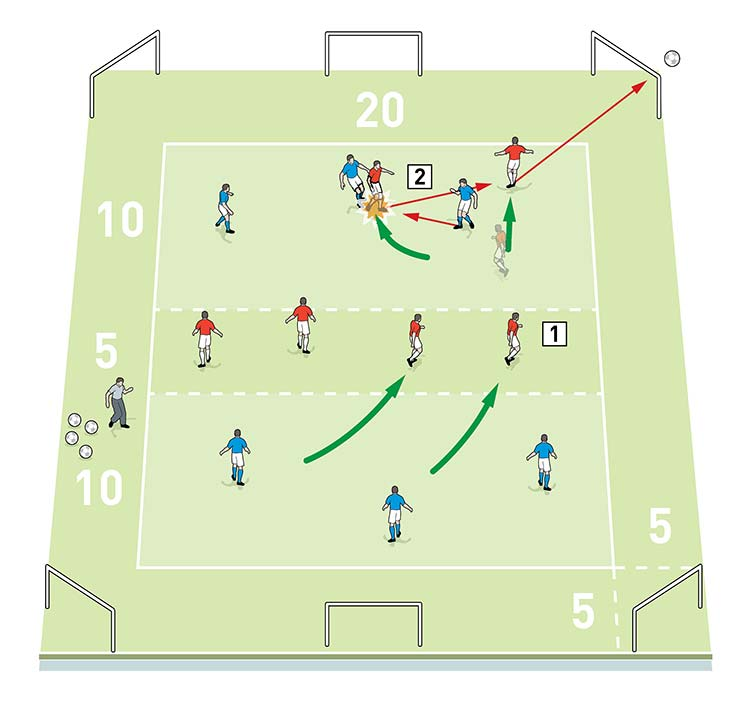
\includegraphics[width=\textwidth]{../img/Trimmed/Press_Protect_2}
    \end{minipage}
    \hspace{0.05\linewidth}
    \begin{minipage}{.5\linewidth} % Left column and width
        \textbf{Drill Description:}
        A drill that focuses on pressing and quick decision making for the passing team.  It also works on showing the importance of the center field player in their role of blocking through balls.
        
        \begin{enumerate}
        \setlength{\itemsep}{0pt}
        \setlength{\parskip}{0pt}
        \setlength{\parsep}{0pt}
        \item 20x25 yard area with a 5 yard middle zone.
        \item The pressing team of 6 stage in the middle, the other team (defending team) splits into 2 groups of 3 in on 10x20 side areas.
        \item 6 goals are positioned around 5 yard outside the area - the pressing team can score by passing the ball through any of these 6 goals.
        \item Coach is on the side line passing balls in.
        \item The pressing team is trying to score goals.
        \item The defending team is playing keep away and can pass to the other side.  At which point the press has to return to the center box 2 other players from the center box come out to press the other side.
        \item Switch roles every 5 minutes or 1/4 of the allocated time.
        \end{enumerate}

        \textbf{Coaching Points:}
        \begin{enumerate}
        \setlength{\itemsep}{0pt}
        \setlength{\parskip}{0pt}
        \setlength{\parsep}{0pt}
        \item Make quick passes.
        \item Think where should I pass the ball all the time (especially when the ball is not at your feet).
        \end{enumerate}
    \end{minipage}
\end{minipage}

\end{evenBlock}


\section{Close}

NO SPRINTS!!!!

\end{document}